\documentclass{extarticle}
\usepackage{graphicx} %
\usepackage{tikz}
\usepackage{amsmath}
\usetikzlibrary{arrows}
\graphicspath{ {./img/} }
\usepackage{geometry}
\geometry{
a4paper,
total={170mm,257mm},
left=20mm,
top=20mm,
}

\title{Rational Algebra}
\author{Gilbran Mahdavikia Raja}
\date{5025241134 $|$ SBD C}

\begin{document}

\maketitle

\begin{enumerate}
% 1
\item {\textbf{Select Nama, Alamat, and Gaji from employee in “Research” department.}}
\begin{description} 
    % \item[$\Leftrightarrow$] {\large Employee\_Department $\leftarrow Employee \bowtie Department$}
    % \item[$\Leftrightarrow$] {\large Employee\_Research $\leftarrow \sigma{\scriptstyle Dname="Research"}(Employee \bowtie Department)$}
    \item[$\Leftrightarrow$] {\large $\pi {\scriptstyle nama,alamat,gaji}(\sigma{\scriptstyle Dname="Research"}(Employee \bowtie Department))$}   
    \item[] 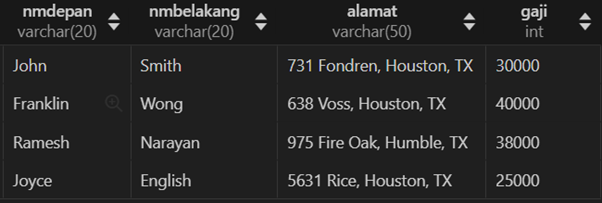
\includegraphics[scale=0.7]{1.png}
\end{description}

% 2
\item {\textbf{Select nama, alamat, and noKTP from employee that is a supervisor of other employees.}}
\begin{description} 
    % \item[$\Leftrightarrow$] {\large Supervisor $\leftarrow \sigma{\scriptstyle NoKTP in NOKTP_MGR}(Employee)$}
    \item[$\Leftrightarrow$] {\large $\pi {\scriptstyle NmDepan,NmBelakang,Alamat,NoKTP}(\sigma{\scriptstyle NoKTP \;IN \; NOKTP\_MGR}(Employee))$}   
    \item[] 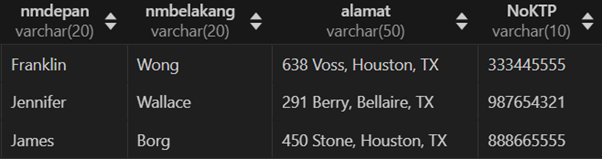
\includegraphics[scale=0.7]{2.png}
\end{description}

% 3
\item {\textbf{Select nama and noKTP from employee with its supervisor’s nama and noKTP.}}
\begin{description} 
    % \item[$\Leftrightarrow$] {\large Employee\_Supervisor $\leftarrow Employee \bowtie {\scriptstyle Employee.NoKTPKepala = Employee.NoKTP}$}
    \item[$\Leftrightarrow$] {\large $\pi {\scriptstyle Nama\_Employee,NoKTP\_Employee,Nama\_Supervisor,NoKTP\_Supervisor}\\(Employee \bowtie {\scriptstyle Employee.NoKTPKepala = Employee.NoKTP})$}   
    \item[] 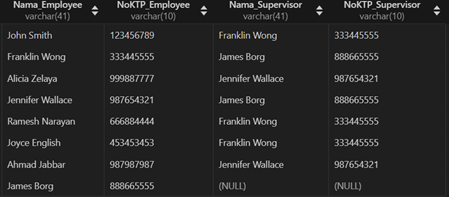
\includegraphics[scale=0.7]{3.png}
\end{description}

% 4
\item {\textbf{Select nama, alamat, and noKTP that is a manager in Department 4.}}
\begin{description} 
    % \item[$\Leftrightarrow$] {\large Department\_Manager $\leftarrow Department \bowtie {\scriptstyle Department.NOKTP\_MGR = Employee.NoKTP}$}
    \item[$\Leftrightarrow$] {\large $\pi {\scriptstyle Nama,Alamat,NoKTP}(\sigma{\scriptstyle Dnomor = 4}(Department \bowtie {\scriptstyle Department.NOKTP\_MGR = Employee.NoKTP}))$}   
    \item[] 
\includegraphics[scale=0.7]{4.png}
\end{description}

\pagebreak

% 5
\item {\textbf{Select nama, alamat, and nama\_proyek from employee that works in "ProductZ" project.}}
\begin{description} 
    % \item[$\Leftrightarrow$] {\large Employee\_Project $\leftarrow Bekerja\_Pada \bowtie {\scriptstyle Bekerja\_Pada.NoKTP = Employee.NoKTP} \bowtie \\ {\scriptstyle Bekerja\_Pada.Pnomor = Project.Pnomor}$}
    \item[$\Leftrightarrow$] {\large $\pi {\scriptstyle Nama,Alamat,Nama_Proyek}(\sigma{\scriptstyle Nama\_Proyek = "ProductZ"}\\(Bekerja\_Pada \bowtie {\scriptstyle Bekerja\_Pada.NoKTP = Employee.NoKTP} \bowtie \\ {\scriptstyle Bekerja\_Pada.Pnomor = Project.Pnomor}))$}    
    \item[] 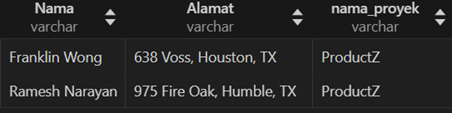
\includegraphics[scale=0.7]{5.png}
\end{description}

% 6
\item {\textbf{Select nama\_proyek controlled by “Research” department.}}
\begin{description} 
    % \item[$\Leftrightarrow$] {\large Department\_Project $\leftarrow Project \bowtie {\scriptstyle Project.Dnum = Department.Dnomor}$}
    \item[$\Leftrightarrow$] {\large $\pi {\scriptstyle Nama_Proyek}(\sigma{\scriptstyle Dname = "Research"}(Project \bowtie {\scriptstyle Project.Dnum = Department.Dnomor}))$}    
    \item[] 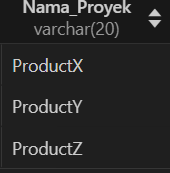
\includegraphics[scale=0.7]{6.png}
\end{description}

% 7
\item {\textbf{Select nama\_proyek located in “Houston” or” Stafford”.}}
\begin{description} 
    % \item[$\Leftrightarrow$] {\large Department\_Project $\leftarrow Project \bowtie {\scriptstyle Project.Dnum = Department.Dnomor}$}
    \item[$\Leftrightarrow$] {\large $\pi {\scriptstyle Nama\_Proyek}(\sigma{\scriptstyle Plokasi = "Houston" \; OR \; Plokasi = "stanfford'}(Project))$}    
    \item[] 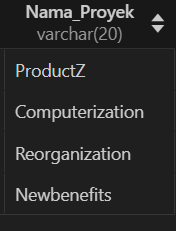
\includegraphics[scale=0.7]{7.png}
\end{description}

% 8
\item {\textbf{Select name and location of the project which “John” work on it.}}
\begin{description} 
    % \item[$\Leftrightarrow$] {\large Employee\_Project $\leftarrow Bekerja\_Pada \bowtie {\scriptstyle Bekerja\_Pada.NoKTP = Employee.NoKTP} \bowtie \\ {\scriptstyle Bekerja\_Pada.Pnomor = Project.Pnomor}$}
    \item[$\Leftrightarrow$] {\large $\pi {\scriptstyle Nama_Project,Location}(\sigma{\scriptstyle NmDepan = "John"}(Bekerja\_Pada \bowtie \\{\scriptstyle Bekerja\_Pada.NoKTP = Employee.NoKTP} \bowtie  {\scriptstyle Bekerja\_Pada.Pnomor = Project.Pnomor}))$}    
    \item[] 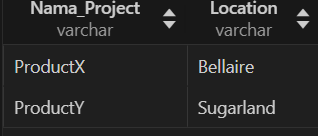
\includegraphics[scale=0.7]{8.png}
    \end{description}
    
    % 9
    \item {\textbf{Select nama and alamat of male employee with salary less than 40000}}
    \begin{description} 
        \item[$\Leftrightarrow$] {\large $\pi {\scriptstyle Nama,Alamat}(\sigma{\scriptstyle JenisKelamin = "L" AND \; Gaji < 40000}(Employee))$}    
        \item[] 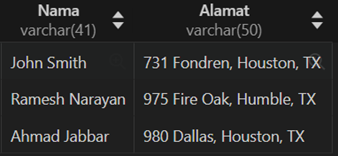
\includegraphics[scale=0.7]{9.png}
    \end{description}
    
        \pagebreak

% 10
\item {\textbf{Select nama and gaji of “Administration” department
manager.}}
\begin{description} 
    % \item[$\Leftrightarrow$] {\large Department\_Manager $\leftarrow Department \bowtie {\scriptstyle Department.NOKTP\_MGR = Employee.NoKTP}$}  
    \item[$\Leftrightarrow$] {\large $\pi {\scriptstyle Nama,Gaji}(\sigma{\scriptstyle Dname = "Administration"}(Department \bowtie \\ {\scriptstyle Department.NOKTP\_MGR = Employee.NoKTP}))$}    
    \item[] 
\includegraphics[scale=0.7]{10.png}
    \end{description}
\end{enumerate}

\end{document}